\section{Testen}

Het is belangrijk dat bepaalde eigenschappen van de gemaakte sensormodule goed getest worden. In dit hoofdstuk worden vier tests beschreven die zijn gedaan om te bepalen of de sensormodule goed functioneert. Hiervoor zijn er bepaalde materialen nodig. Voor de eerste twee tests zijn de materialen uit \cref{tab:testMaterialen} gebruikt. De andere tests gebruiken de materialen uit \cref{tab:testMaterialen2}.

\begin{table}[ht]
    \centering
    \begin{tabular}{l|l|l}
        Apparaat         & Serienummer & Beschrijving \\
        \hline
        MSREF1           & 23/RS03     & Referentie elektrode       \\
        MSFET 3330-2     & 23/205      & ISFET pH sensor            \\
        Tektronix MSO 46 & C019070     & Oscilloscoop               \\
        uitlees PCB      & 1           & ISFET uitlees schakeling   \\
        voeding PCB      & 1           & BMS en energy harvester    \\    
        \hline
    \end{tabular}
    \caption{Materialen die zijn gebruikt voor de tests}
    \label{tab:testMaterialen}
\end{table}

\subsection{Stabiliteitstest}
De eerste test is bedoelt om te controleren of de uitgang van de opamp stabiel is. Dit is een belangrijke test om uit te voeren. Als de uitgang namelijk niet stabiel is, zal de spanning die de ADC uitleest niet goed overeen komen met de drempelspanning van de ISFET.

Om de test uit te voeren wordt de uitlees PCB verbonden met de voeding PCB, zodat de uitleesschakeling een voeding heeft. De probe van kanaal 1 van de oscilloscoop wordt verbonden met de uitgang van de opamp. De probe van kanaal 2 wordt verbonden met de drain van de ISFET. De ISFET wordt samen met de referentieelektrode in een pH 7 bufferoplossing gestopt. De opstelling is in \cref{fig:test ISFET circuit best} schematisch te zien.

\begin{figure}[ht]
    \centering
    \def\svgwidth{0.75\textwidth}
    \input{img/ISFETCircuitBestTest.pdf_tex}
    \caption{De locatie van de scope probes in de schakeling om te testen of de uitgang stabiel is.}
    \label{fig:test ISFET circuit best}
\end{figure}


\subsubsection{Resultaten} \label{sec:stabilityTestResults}

De eerste test resulteerde in een oscillerend signaal. De uitgang van de opamp gaf een signaal dat elke \qty{6.8}{\milli\second} pulseerde. Dit is te zien in \cref{fig:resultUgsUds}.
Wanneer de opamp uitgang laag is, waardoor de gate-source spanning op de ISFET 0 V wordt, komt de drain-source spanning van de ISFET erg langzaam omhoog. Wanneer deze spanning boven de referentiespanning komt, gaat de uitgang van de opamp omhoog, waarna de drain-source spanning van de ISFET erg snel begint te dalen. Echter, wanneer de drain-source spanning vervolgens de referentiespanning bereikt, reageert de opamp hier merkwaardig genoeg niet direct op. Dit zorgt voor een oscillerende werking. Ditzelfde resultaat kwam uit dezelfde test met een andere opmamp (de MCP6002).

Op de drain-source spanning is ook een tweede oscillatie met een hogere frequentie zichtbaar.


% Een mogelijke reden hiervoor is dat de ISFET niet snel genoeg reageert op spanningsveranderingen tussen de gate (de referentie elektrode) en de source. 

% 

% Dit wordt waarschijnlijk veroorzaakt door de interne chopping van de gekozen opamp.

\begin{figure}[ht]
    \centering
    \def\svgwidth{0.75\textwidth}
    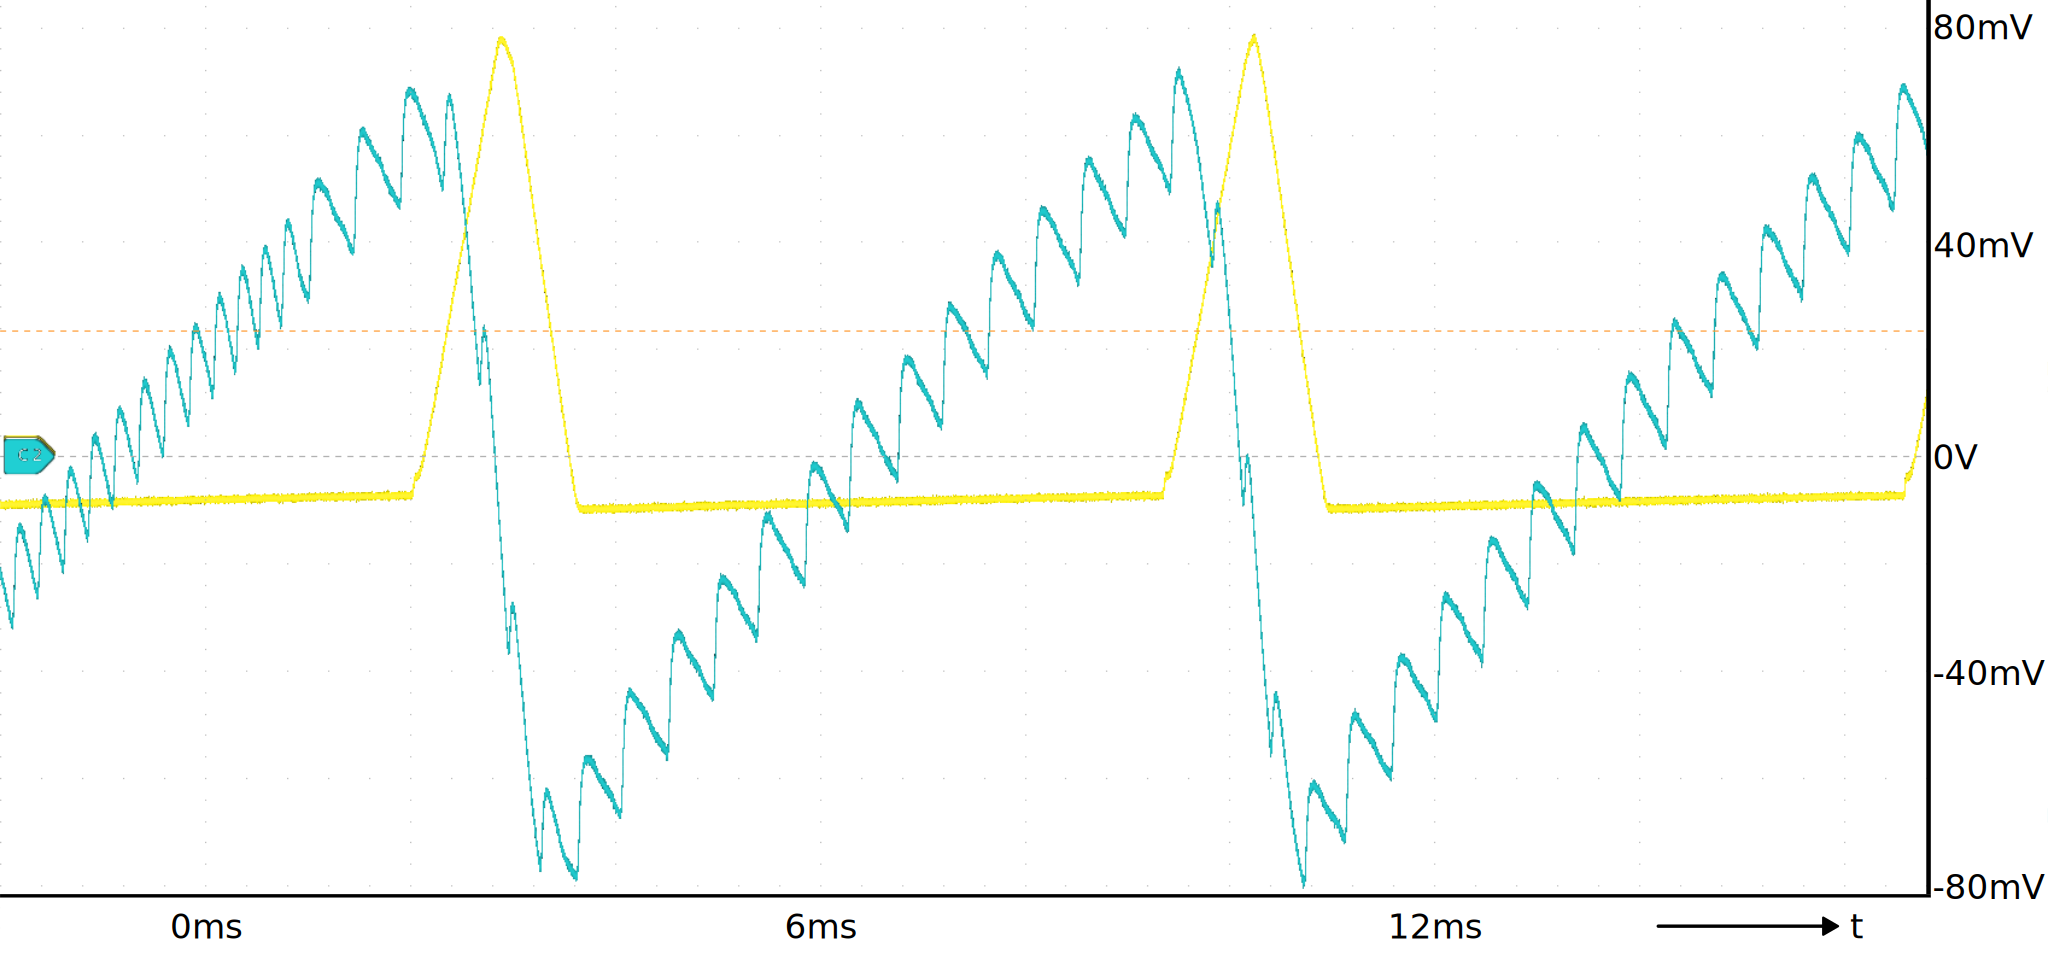
\includegraphics[width=0.8\textwidth]{testUgsUds.png}
    \caption{Het resultaat van de stabiliteitstest. Kanaal 1 (geel) is $U_{gs}$, kanaal 2 (lichtblauw) is $U_{ds}$.}
    \label{fig:resultUgsUds}
\end{figure}


\subsubsection{Discussie}
Er zijn meerdere mogelijke oplossingen voor de instabiliteit.
Eén mogelijke oplossing is een integrator plaatsen tussen de uitgang van de opamp en de gate van de ISFET. Dit zou ervoor zorgen dat de ISFET genoeg tijd heeft om te reageren op de veranderde gate-source spanning, waardoor deze de opamp kan bijhouden.

Een andere mogelijke oplossing is een RC-filter te plaatsen tussen de drain van de ISFET en de niet-inverterende ingang van de opamp. Dit zorgt ervoor dat de opamp trager gaat werken, waardoor de ISFET de opamp bij kan houden.

Er zal een aantal tests gedaan moeten worden om te vinden hoe de ISFET precies reageert op een verandering van de gate-source spanning, en hoe dit verschilt van een reguliere MOSFET. Zo kan een beter model opgesteld worden van de ISFET, waar dan vervolgens een betere uitleesschakeling mee ontworpen kan worden.


\subsection{pH waarde test} 
De volgende test is bedoelt om te testen of het uitgangssignaal verandert op basis van de pH waarde. 

Om te beginnen wordt de uitlees PCB verbonden met de voeding PCB, zodat de uitleesschakeling gevoed wordt. De probe van kanaal 1 van de oscilloscoop wordt verbonden met de ingang van de ADC. De probe van kanaal 2 wordt verbonden met de uitgang van de opamp. Vervolgens worden de ISFET en referentieelektrode in een pH 7 bufferoplossing gestopt. De golfvorm die de oscilloscoop geeft kan nu worden opgeslagen. De meting wordt herhaalt met de ISFET en referentieelektrode in een pH 4 bufferoplossing.

\subsubsection{Resultaten}
De resultaten van deze test zijn te zien in \cref{fig:resultspHMeasure}. Duidelijk is de amplitude van de uitgang van de opamp hoger op pH 7 vergeleken met pH 4.

\begin{figure}[ht]
    \centering
    \begin{subfigure}[b]{0.475\textwidth}
        \centering
        \def\svgwidth{\textwidth}
        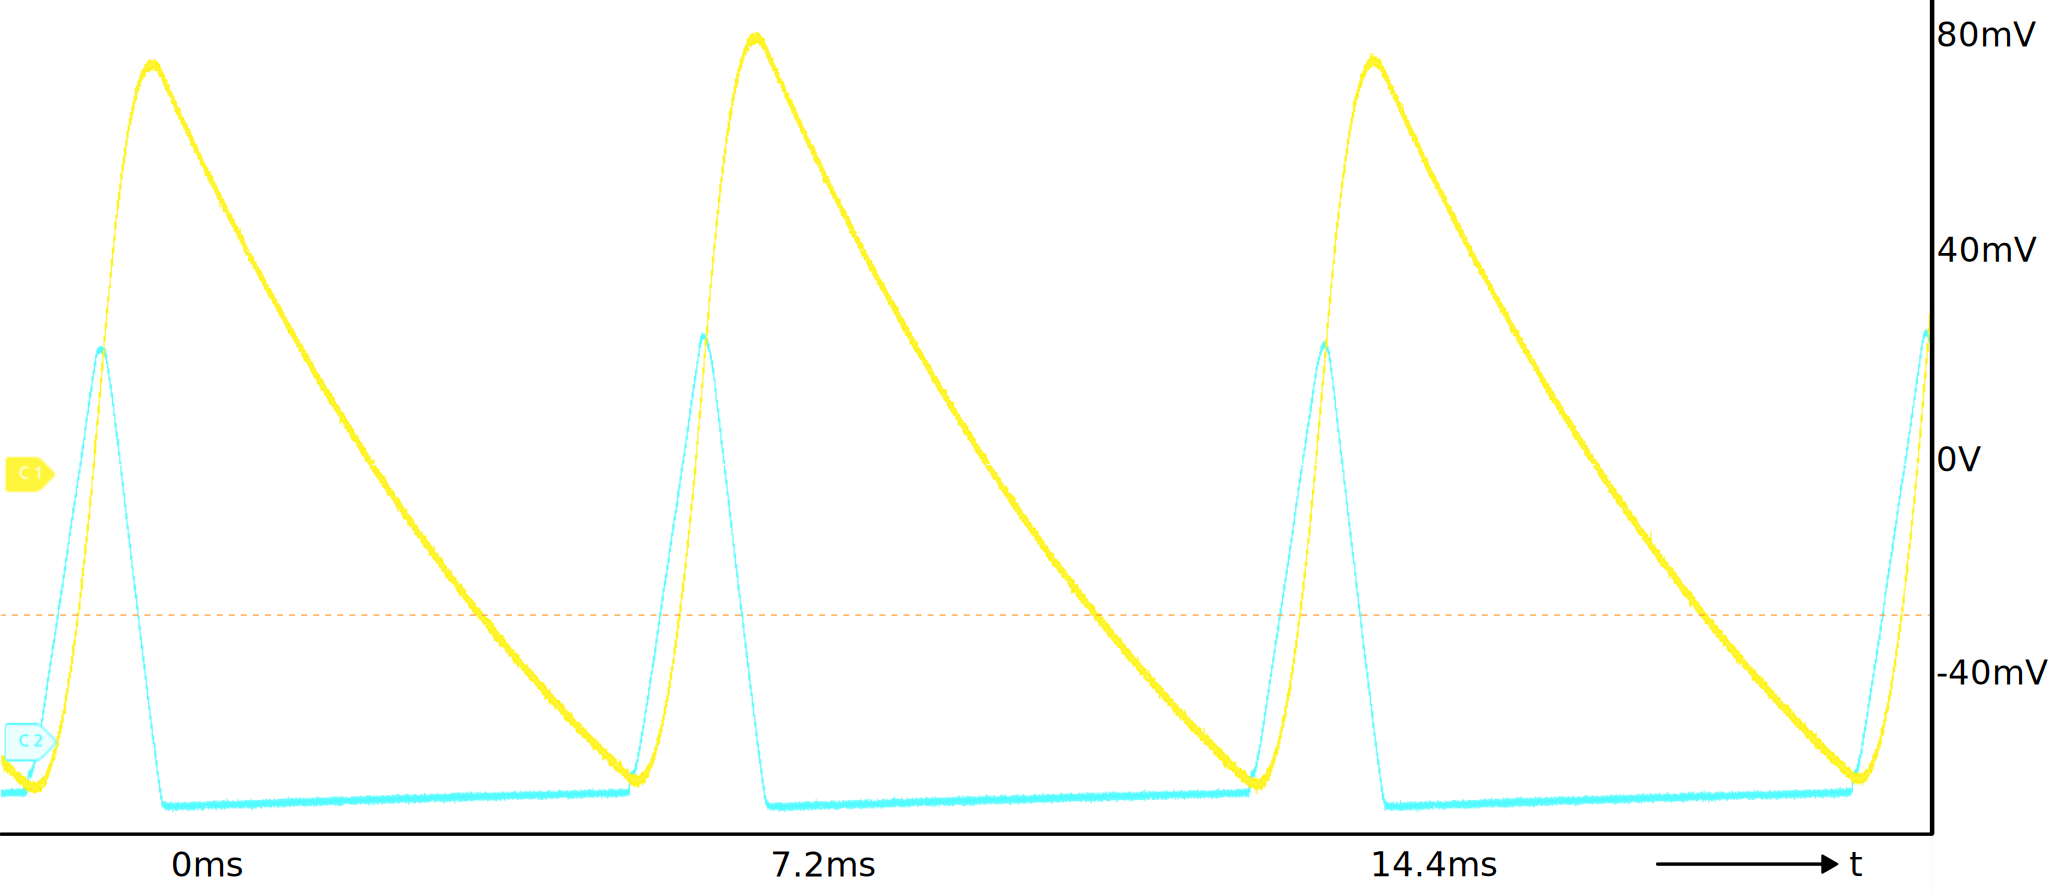
\includegraphics[width=\textwidth]{testpH7.png}
        \caption{De uitgang van de opamp (lichtblauw) en ingang van de ADC (geel) op pH 7.}
        \label{fig:resultpH7}
    \end{subfigure}
    \hfill
    \begin{subfigure}[b]{0.475\textwidth}
        \centering
        \def\svgwidth{\textwidth}
        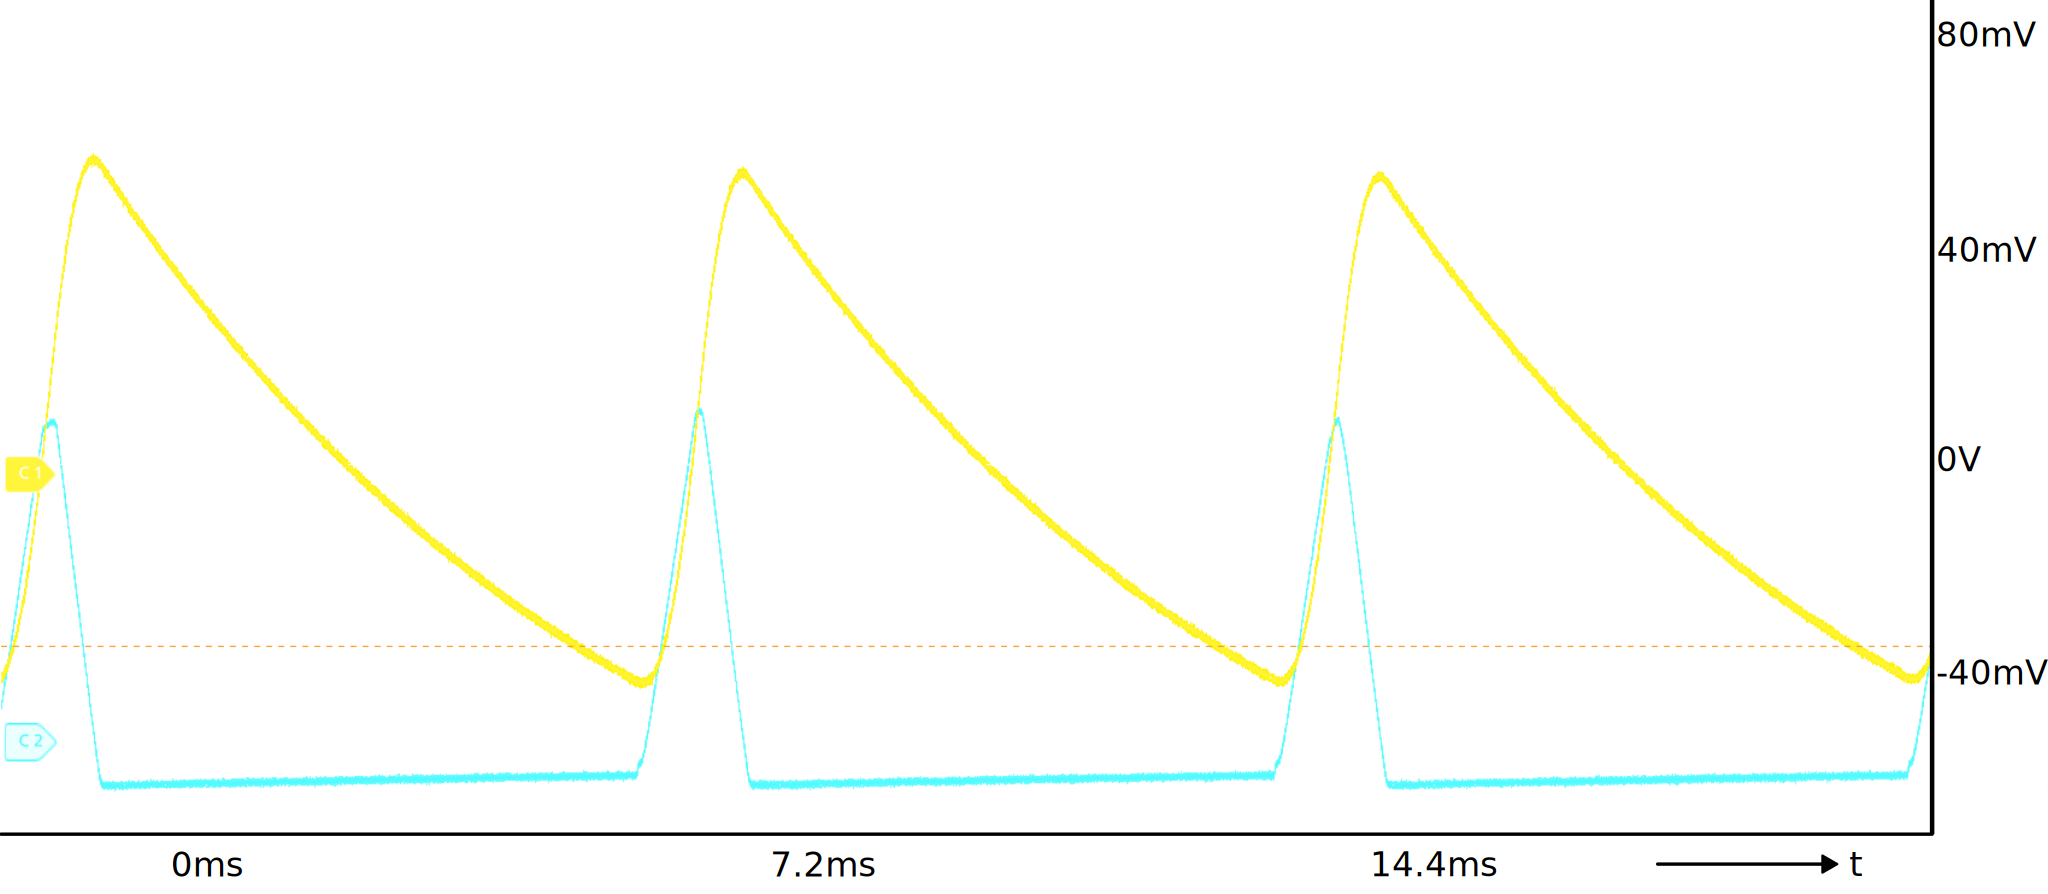
\includegraphics[width=\textwidth]{testpH4.png}
        \caption{De uitgang van de opamp (lichtblauw) en ingang van de ADC (geel) op pH 4.}
        \label{fig:resultpH4}
    \end{subfigure}
    \caption{De uitgang van de meetschakeling op pH 4 en pH 7. Beide metingen hebben dezelfde schaal.}
    \label{fig:resultspHMeasure}
\end{figure}

\subsubsection{Discussie}
Een verandering van pH waarde heeft duidelijk een effect op het uitgangssignaal. Er kan echter nog weinig gezegd worden over de lineariteit van de uitgang op basis van de pH waarde. Hiervoor zou de uitgang eerst stabiel gemaakt moeten worden.


\begin{table}[ht]
    \centering
    \begin{tabular}{l|l|l}
        Apparaat         & Serienummer & Beschrijving \\
        \hline
        MSREF1           & 23/RS03     & Referentie elektrode       \\
        MSFET 3330-2     & 23/205      & ISFET pH sensor            \\
        uitlees PCB      & 1           & ISFET uitlees schakeling   \\
        voeding PCB      & 1           & BMS en energy harvester    \\    
        Keithley DMM6500 & 04458071    & Multimeter spanningsmeting \\
        Keithley DMM6500 & 04458625    & Multimeter stroommeting    \\
        \hline
    \end{tabular}
    \caption{Materialen die zijn gebruikt voor de tests}
    \label{tab:testMaterialen2}
\end{table}


\subsection{Vermogen test}
Deze test is bedoelt om te controleren of het volledige systeem minder dan 10 mW aan vermogen gebruikt. Dit is gedaan door de batterij spanning te meten en de stroom die uit de batterij richting het gehele systeem gaat. Daarvoor zijn 2 Keithley mutlimeters gebruikt. Eén ingesteld op stroom meting modus en geplaatst zodat de batterijstroom door de multimeter gaat. De andere Keithley multimeter is ingesteld om spanning over de batterij klemmen te meten. 

\subsubsection{Resultaten}
De gemeten batterijspanning was 3.82 V, tijdens de loop van de test was deze constant. Het stroomverbruik is tijdens het normaal functioneren van het systeem gemeten tussen 1.3 mA en 2.5 mA. De gemeten stroomwaardes zijn vermenigvuldigd met 3.82V en vervolgens geplot. Deze plot is te zien in \cref{fig:vermogenMeting}. Daarnaast is er een gemiddelde genomen van alle samples om het gemiddelde vermogen te kunnen berekenen. Het gemiddelde vermogen is uitgekomen op 6.81 mW. 

\begin{figure}[ht]
    \centering
    \includegraphics[width=\textwidth]{img/vermogensMeting.pdf}
    \caption{Vermogen meting van systeem}
    \label{fig:vermogenMeting}
\end{figure}

\subsubsection{Discussie}
Uit de metingen is duidelijk te zien dat het hele systeem minder vermogen verbruikt dan de maximale 10 mW die genoemd is in de \cref{sec:systemSpecifications}. 


\subsection{Energy harvesting test}
Voor de energy harvesting test is er een meetopstelling gebruikt waarbij de stroom van en naar de accu gemeten wordt. Vervolgens is het piëzo-element aangesloten op de energy harvesting PCB. Dit element is door middel van een magneet aan de tip van het piëzo-element aan een boormachine kop vastgemaakt. Dit zorgde ervoor dat het piëzo-element bij het draaien van de boormachine vibreerde. Bij deze test is alleen de voeding PCB aanwezig en is de uitlees PCB niet aangesloten.

\subsubsection{Resultaten}
De meting is geëxporteerd en omgezet naar mW, door de gemeten stroom te vermenigvuldigen met de batterijspanning. Dit is zien in \cref{fig:vermogenPlot}.

\begin{figure}[ht]
    \centering
    \includegraphics[width=\textwidth]{vermogen_tijd_plot.pdf}
    \caption{Vermogen meting energy harvesting}
    \label{fig:vermogenPlot}
\end{figure}

\subsubsection{Discussie}
In \cref{fig:vermogenPlot} is te zien dat het energieverbruik van de accu naar 0 mW gaat zodra het piëzo-element genoeg vibreert. Dit toont aan dat de energy harvesting werkt en op lange termijn de levensduur van de sensormodule zal verlengen.